\documentclass[conference]{IEEEtran}
\IEEEoverridecommandlockouts
% The preceding line is only needed to identify funding in the first footnote. If that is unneeded, please comment it out.
\usepackage{cite}
\usepackage{amsmath,amssymb,amsfonts}
\usepackage{algorithmic}
\usepackage{float}
\usepackage{graphicx}
\usepackage{textcomp}
\usepackage{xcolor}
\newcommand{\argmax}[1]{\underset{#1}{\operatorname{arg}\,\operatorname{max}}\;}
\newcommand{\argmin}[1]{\underset{#1}{\operatorname{arg}\,\operatorname{min}}\;}
\def\BibTeX{{\rm B\kern-.05em{\sc i\kern-.025em b}\kern-.08em
    T\kern-.1667em\lower.7ex\hbox{E}\kern-.125emX}}
\begin{document}

\title{Application of Supervised Learning in Stop Sign Detection}


\author{\IEEEauthorblockN{Joseph Bell}
\IEEEauthorblockA{\textit{Department of Electrical and Computer Engineering} \\
\textit{University of California, San Diego}\\
jjbell@eng.ucsd.edu}
}

\maketitle

\begin{abstract}
This paper presents a supervised learning approach to stop sign detection through the method of discriminative classification via a logistic model. The logistic model functions as a probabilistic color model that aims to classify pixels into two classes: red and not red. The results of this approach were respectable - achieving a 67 percent success rate on a set of curated test images.
\end{abstract}

\begin{IEEEkeywords}
supervised learning, logistic regression, stop sign detection
\end{IEEEkeywords}

\section{Introduction}

In April 2016 the Dubai Autonomous Transportation Strategy was introduced with the goal of converting 25 percent of all transportation to be autonomous by 2030 [1]. With the recent explosion in autonomous driving research, stop sign detection is one of many problems these autonomous vehicles face. Autonomous driving is quite frankly a paradigm shift in the realm of transportation, and safety, more specifically the ability to detect traffic signs, is a critical concern to many that comes with the implementation of autonomous driving. A 2018 Allianz Global Assistance Survery [2] shows that 57 percent of Americans are not interested in utilizing autonomous vehicles (up from 47 percent the previous year), and that 71 percent (up from 65 percent the previous year) of the uninterested group cited safety concerns when asked for the motivation behind their disinterest. It is clear that safety is at the forefront of peoples' minds with the implementation of autonomous vehicles, and algorithms that can confidently detect traffic signs are non-negotiable. 

The goal of this paper is to detail an approach to applying a supervised learning algorithm for stop sign detection by use of a logistic regression model. Training data was curated from a set of training images and two classes of pixels were assigned labels: pixels that came from a stop sign and pixels that did not come from a stop sign. This paper will first introduce the problem formulation before traversing to the technical approach and methods of solving the problem. Lastly, results of the supervised learning model will be presented and discussed.

\section{Problem Formulation}

Given a set of training images, a data set needs to be created such that $D = \{x_{i}, y_{i}\}^{n}_{i=1}$ where $x_{i}$ represents a 3x1 vector of pixel values and $y_{i}$ represents the pixel's scalar label. Using the data set of pixel values and labels, a probabilistic color model needs to be built that is capable of classifying the pixels of an input image into their respective color class.

After an image's pixels have been classified into their respective classes, a method for shape detection must be implemented. The method needs to be able to detect if a group of pixels in the red class resembles the shape of a stop sign or not by use of shape statistics and other higher-level features. Once a group of pixels in the red class has been determined to resemble the shape of a stop sign, a bounding box is to be drawn around it. The final output is to be the original image with bounding boxes drawn around any stop sign present in the image. 

\section{Technical Approach}

\subsection{Approach to Training Data}

The training data was curated using roipoly [3] to select regions of interest (the stop signs) and create binary masks where white corresponds to the stop sign region and black corresponds to everything else. Figure 1 illustrates a training image and its corresponding binary mask.
\begin{figure}[H]
\centerline{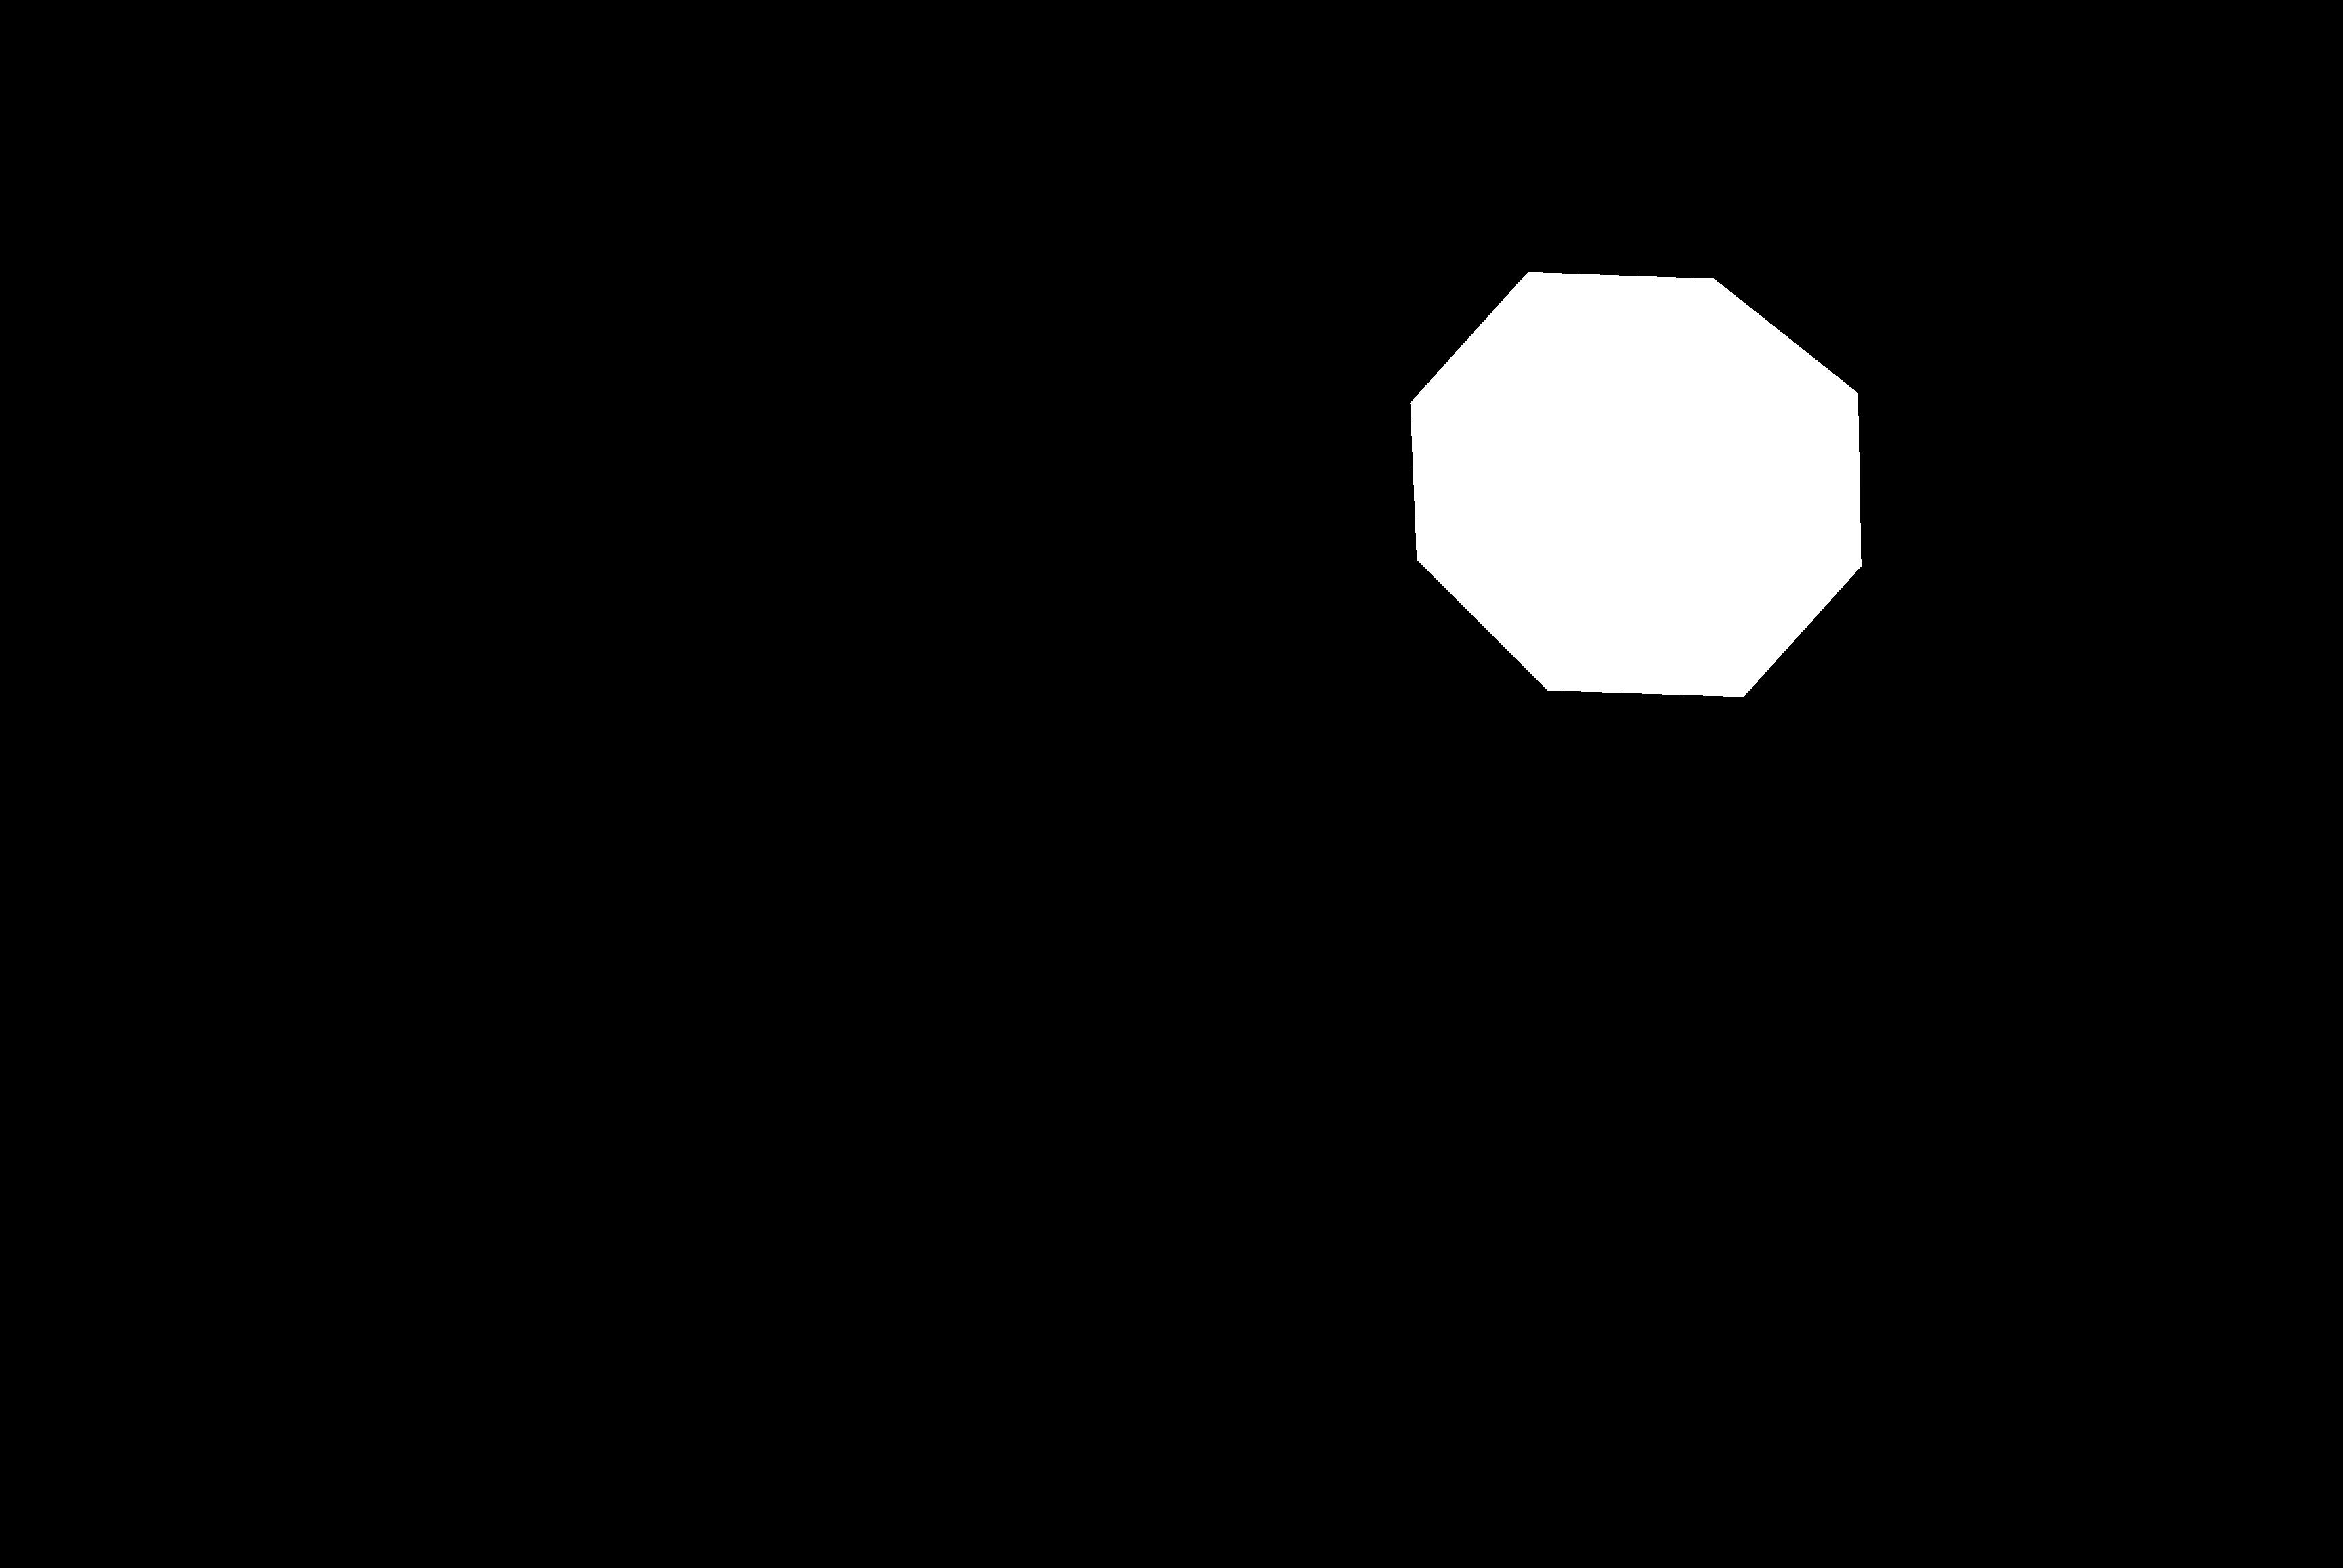
\includegraphics[width=30mm]{2mask.jpg}
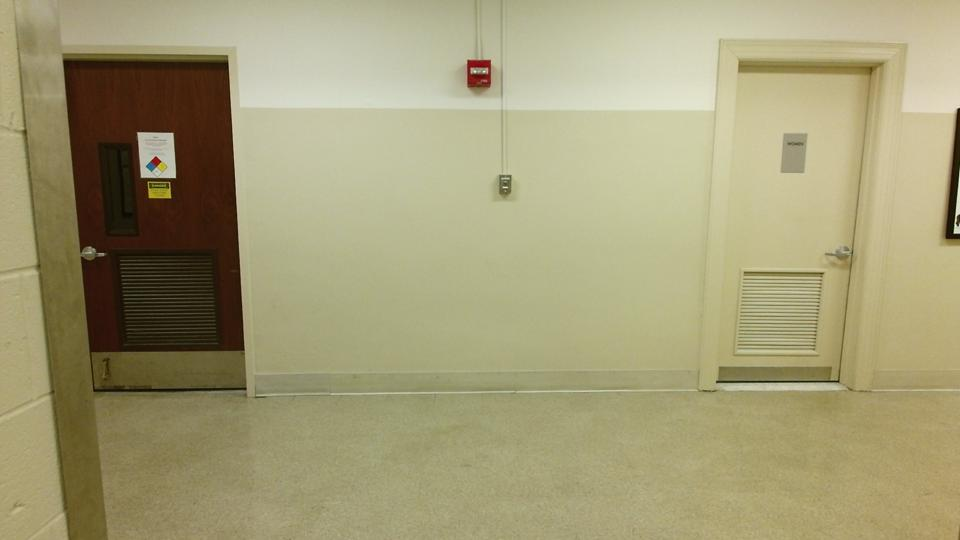
\includegraphics[width=30mm]{2.jpg}}
\caption{Training image with corresponding binary mask generated with roipoly}
\end{figure}

76 total training images and binary masks were curated, however only 40 were used due to computation time and high resolution images (above 1,000 kilobytes) were not included in the set of 40 training images selected. For efficient computation, the data set is converted to the form $D = \{X,\textbf{y} \}$ where $X \in \mathbb{R}^{nx3} $ and $\textbf{y} \in \mathbb{R}^{n}$. More specifically, training images were reshaped from 3-D $(n,m,3)$ arrays to 2-D $(n*m,3)$ where n represents rows and m represents columns of the input training image. The reshaped array was then appended row-wise to an array containing the cumulative total of pixel training data. The result is a 2-D array of the form $(p,3)$ where each row of the p dimension is a data point and the 3 columns are the pixel values. The masks were similarly reshaped, but from a 2-D array of the form $(m,n)$ to $(m*n,1)$ and appended row wise to an array containing the cumulative total of pixel labels. Stop sign pixels were assigned the scalar value of 1 as a label and all other pixels were assigned the scalar value of -1 as a label. The reasoning behind these label values is discussed in the section regarding color segmentation.

\subsection{Approach to Color Spaces}

The classification was attempted in RGB and YCbCr color spaces. The motivation behind attempting to use different color spaces came from mapping a training image into different color spaces and observing the plots. An example is shown in Figure 2 where a training image is plotted in both the RGB and YCbCr color space. Upon visualization the assumption was made that the YCbCr colorspace would out-perform the RGB color space classification due to the more discriminant groupings of the color pixels; the bulk of red pixels in the YCbCr color space seem to have a larger L2 norm between pixels of other colors. However, to determine which color space to use for the full set of training images, a test run of image segmentation after learning parameters from the data points of 5 training images was performed. The RGB color space out performed the YCbCr color space, and therefore the RGB colorspace was used for the full set of 40 training images.

\begin{figure}[H]
\centerline{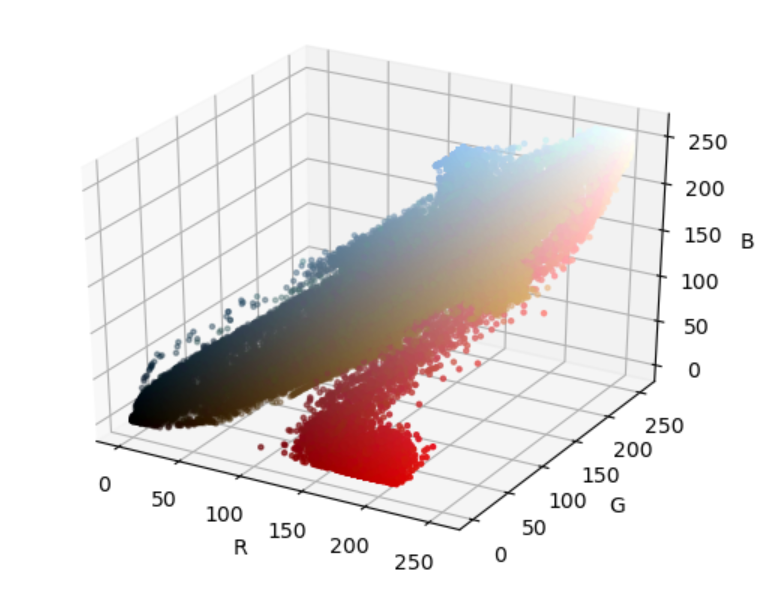
\includegraphics[width=50mm]{rgb.png}
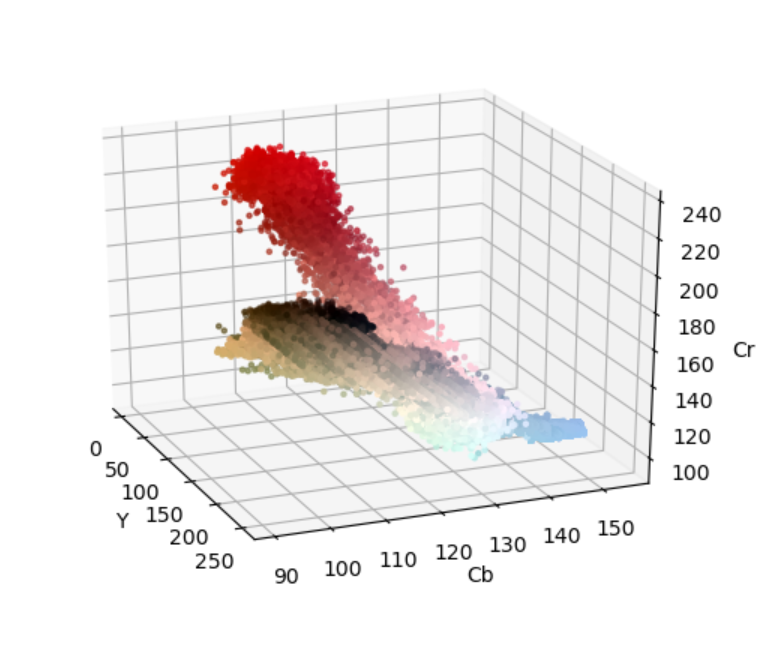
\includegraphics[width=50mm]{ycrcb.png}}
\caption{Color space visualizations of the RGB and YCbCr from left to right }
\end{figure}

\subsection{Approach to Color Segmentation}

A supervised learning, logistic regression, probabilistic color model was designed via the sigmoid function to classify pixels into two classes: red and not red. The color classifier takes an input image and returns a binary image of 1s for red pixels and 0s for every other color.

The sigmoid function used to map the pixel values to a space for discriminant analysis is:
\[\sigma(z) = \frac{1}{1+exp(-z)}, z = y\omega^Tx\]
Where $\omega$ is the vector of parameters to learn, y is the scalar label, and x is the pixel color vector.
In order for this function to be modeled as a probability distribution, the sum of all probabilities must equate to 1. Due to the binomial nature of this classification approach, the probability of a stop sign pixel is represented as $\sigma(z)$ and the probability of the pixel not being a stop sign is represented as $1 - \sigma(z)$. The labels being 1 or -1 is used as an advantage as the sigmoid function has nice properties in which $1 - \sigma(z) = \sigma(-z)$, thus resulting in $P(y=1|x,\omega) = \sigma(1*\omega^Tx) = \sigma(z)$ and $P(y=-1|x,\omega) = \sigma(-1*\omega^Tx) = \sigma(-z)$. 

Since the data is independent and identically distributed:
\[P(\textbf{y}|X,\omega) = \prod_{i=1}^{n} \sigma(y_{i}x_{i}^T\omega) = \prod_{i=1}^{n} \frac{1}{1+exp(-y_{i}x_{i}^T\omega)}\]

The maximum likelihood estimate was taken for this approach and was found by maximizing the log-likelihood, which equates to minimizing the negative log-likelihood:
\[\omega_{MLE} = \argmax{\omega} logP(\textbf{y}|X,\omega)= \argmin{\omega} \sum_{i=1}^{n} log(1+exp(-y_{i}x_{i}^{T}\omega)) \]

The gradient with respect to $\omega$ does not equal 0 (i.e. there is no closed-form solution) so gradient descent is used in order to iteratively minimize the negative log-likelihood and obtain a global minimum:

\[\omega_{MLE}^{(t+1)} = \omega_{MLE}^{(t)} - \alpha \nabla_{w}(-logP(\textbf{y}|X,\omega)), \omega = \omega_{MLE}^{(t)}\]


The gradient descent equation ultimately simplified to:
\[\omega_{MLE}^{(t+1)} = \omega_{MLE}^{(t)} + \alpha \sum_{i=1}^{n} y_{i}x_{i}(1-\sigma(y_{i}x_{i}^{T}\omega_{MLE}^{(t)}))\]

The final step in the color segmentation problem was to determine a decision boundary - the line where the two classes have equal likelihood:

\[\frac{P(y=1|x_{*},\omega^{*})}{P(y=-1|x_{*},\omega^{*})} = 1 = \frac{1+exp(x_{*}^{T}\omega^{*})}{1+exp(-x_{*}^{T}\omega^{*})} => x_{*}^{T}\omega^{*} = 0\]

Therefore, the decision rule is as follows:

\[y^{*} = \begin{cases} 
      1 & x_{*}^{T}\omega^{*}\geq 0 \\
      -1 & x_{*}^{T}\omega^{*}< 0 
   \end{cases}
\]

Where $\omega^{*}$ is the vector of learned parameters and $x_{*}$ is an image pixel from the input image. An $\alpha$ value of 0.1 was chosen for gradient descent due to simplicity's sake.

Using the learned parameters, new images are read in and a dot product was performed pixel by pixel with the learned parameters to create a segmentation mask in which dot products greater than 0 resulted in a white pixel and dot products less than zero resulted in a black pixel (as per the boundary decision rule). 

The segmented mask was then passed on to the shape detection algorithm, which is discussed in the next section.

\subsection{Approach to Shape Detection}

The high-level description to the approach to shape detection is simply trial and error. A series of criteria were implemented to determine which groups of pixels resembled a stop sign. By analyzing the results of accurate classifications, false positives, and false negatives an optimal combination of criteria was created to develop the final shape detection algorithm.

Four criteria were developed for determining the likelihood that a group of pixels were indeed a stop sign - all four methods are operations performed on the contours of pixel groups. The four criteria were the percent overlap with a minimum-enclosing circle, the area of the contour, the similarity to the Hu invariants of a given octagonal contour, and the percent difference between the major and minor axes of an ellipse fit to the contour. Although not all four criteria were used for the final detection approach, an array of combinations of the four criteria were tested and, through trial and error, an optimal combination was selected for the final detection method. The formulas used to obtain quantitative results for the four criteria are introduced below.

\subsubsection{Percent overlap with a minimum-enclosing circle}

\[v = \frac{A_{contour}}{A_{circle}}\]

\subsubsection{Contour area}

\[x = \sum_{i=1}^{n} 1\]
Where n is the number of pixels inside the contour region.
\subsubsection{Hu invariant comparison}

\[y = \argmax{i=1,2,...7}\frac{|m_{i}^{A}-m_{i}^{B}|}{|m_{i}^{A}|}\] where \[m_{i}^{A} = sign(h_{i}^{A}) \cdot log(h_{i}^{A}) \] \[m_{i}^{B} = sign(h_{i}^{B}) \cdot log(h_{i}^{B}) \] and $h_{i}^{A},h_{i}^{B}$ are the Hu moments for contours A and B, respectively.

\subsubsection{Percent difference between ellipsoid axes}

\[z = \frac{(major - minor)}{major}\]

The OpenCV python library was used extensively for detecting and classifying shapes of the segmentation masks. The initial step was to use the findContours() function which stores (x,y) coordinates that denote the border for a set of white pixels (i.e. pixels that had been classified as red). The contours returned have a multitude of accompanying analysis functions, and the four used for shape detection were minEnclosingCircle(), contourArea(), matchShapes(), and fitEllipse(). Some image segmentations had scatters of false positives, and findContours() would return contours for all of these small patches of white pixels, as shown in Figure 3. However, these noisy regions of pixels were usually small relative to the size of the stop sign of an image. 

\begin{figure}[H]
\centerline{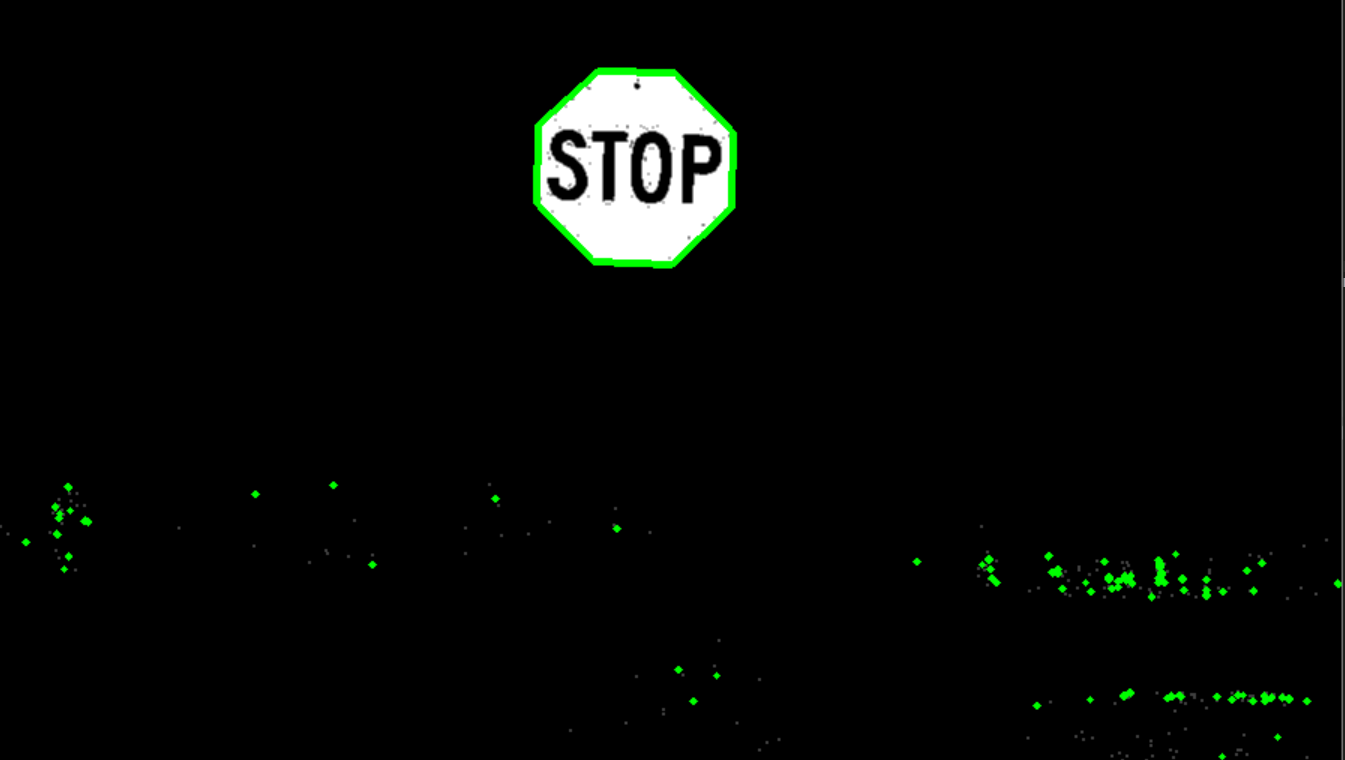
\includegraphics[width=40mm]{noisy_contours.PNG}}
\caption{Example of small detected contour regions relative to a present stop sign}
\end{figure}

The contourArea() function was used to sort the contours by their area (i.e. the number of pixels inside the contour) and the largest contours were stored in a separate list. However, another set of criteria is needed in the case of images that include red objects of substantial size. The minEnclosingCircle(), matchShapes(), and fitEllipse() functions were used after the area sorting to return a metric on what kind of shape the detected contour represents. A stop sign is relatively circular in shape, thus a large portion of a stop sign's contour area is likely to be inside a bounding circle as opposed to that of a telephone pole or car. The metric returned by stop signs in test images was promising as stop sign contours did have significantly higher fractions of their area inside of an enclosing circle than other detected red shapes. However, these large area fractions were only returned when the full face of the stop sign was showing (i.e. the stop sign was not at an angle) as the stop sign would take on a shape more similar to that of an ellipsoid when rotated. The fitEllipse() function proved to be more successful in not only recognizing angled stop signs, but also resulted in less false positives of oddly shaped, but relatively circular contours. Therefore, the use of the minEnclosingCircle() function and criteria 1 for shape detection was deprecated and fitEllipse() and criteria 4 took its place.

Shortly after the deprecation of criteria 1, the deprecation of criteria 3 followed for the same reason. Calculating the percent difference of the major and minor axes allowed for the detection of both ovular and circular shapes by setting an upper limit on the percent difference. Since circles have a percent difference of 0 between their major and minor axes, the magnitude of the returned metric of a contour detailed how ovular the contour is. The only benefit that criteria 3 carried with it was it's ability to match specifically octagonal shapes regardless of scale, but as previously mentioned any rotation of the stop sign about its z-axis (the axis pointing out of the screen) made the stop sign appear ovular and the matchShapes() function used for criteria 3 performed very poorly to this type of rotation. 

The final step that proved beneficial in conjunction with criteria 4 was to approximate a polygon about the contour using the OpenCV approxPolyDp() function which approximates a polygon to a given contour based on its arc length. Small adjustments to the polygon approximation were made until stop sign contours were almost perfectly matched as octagons - Figure 3 depicts a great example of a perfectly octagonal contour. Some contours weren't able to be completely approximated by an octagonal shape, and after yet more trial and error an acceptable range of the number of contour sides was implemented that proved successful in separating stop signs from other false positives that were in the acceptable range for the percent difference of major and minor axes.

\section{Results and Discussion}

Although the trial and error approach to shape detection was not elegant by any means, it did end up providing respectable results. Throughout the process some criteria were found to be unfit for accommodating the fact that stop signs in pictures are not always directly facing the camera - thus affecting their perceived shape. The upper bound on the percent difference of major axes was established at 25 percent and the range of contour edges was established to be between 7 and 18. The learned parameters after 100 iterations of gradient descent on a training set of 18,208,541 data points resulted in [-2.07225554, -8.15944997, 3.54137508] - the convergence plot can be observed below in Figure 4. 

\begin{figure}[H]
\centerline{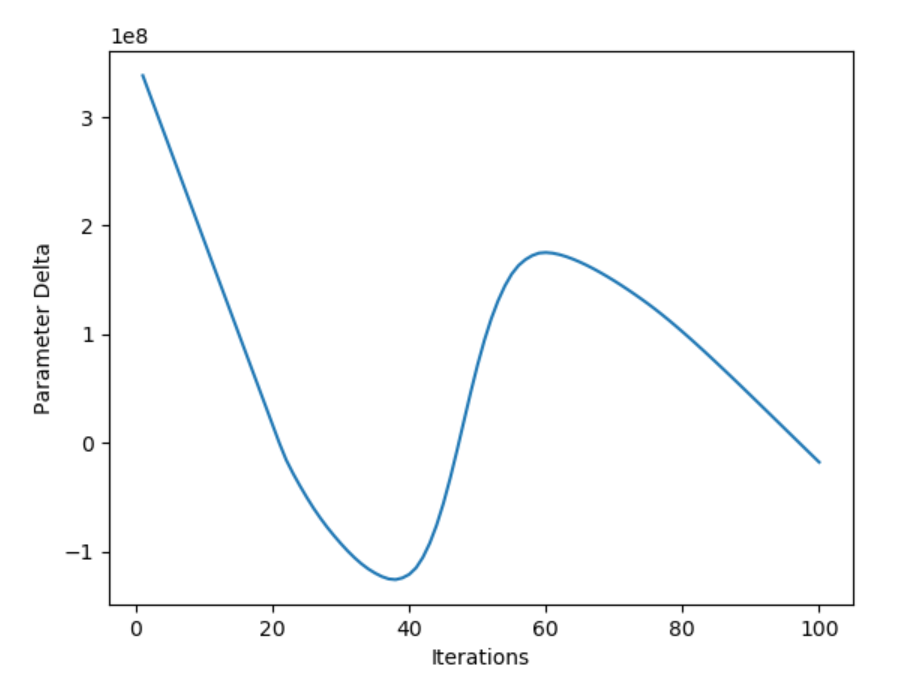
\includegraphics[width=60mm]{convergence.png}}
\caption{Convergence plot of learned parameters}
\end{figure}

The convergence plot measured convergence based off of the sum of differences of the 3 learned parameters between iterations. At approximately 38 iterations it seems that a minimum value for the likelihood function is soon to come to fruition, however the convergence plot makes a detour and ascends. Eventually the plot descends again, but the iteration cap was set at 100 iterations (which was ran over night for 12 hours) and the gradient descent stopped. Had more time been available, or had a more computationally equipped computer been used, the gradient descent could be continued past 100 iterations to see if a final convergence point is met. I predict that a series of oscillations would occur before arriving at a convergence point. Incorporating the use of the Lipschitz constant for $\alpha$ in the gradient descent as opposed to the constant of 0.1 could have resulted in a more efficient gradient descent. Also, regarding the training data, since the "STOP" lettering on the sign is white there were white pixels being labeled as red pixels in the training data as the entire stop sign was selected as the region of interest. However, this noise in the training data did not seem to have much effect on the classifications. It is possible, however, that had there been no noise in the training data there would have been slightly better results in classification.

In test images where the stop sign was a a prominent, front facing feature in the image the detection model detailed in this paper had an approximately 95 percent success rate based on a sample of 20 test images. However, in a more difficult set of 15 images where the stop sign is occluded by the environment, multiple stop signs exist, or circular red objects are present in the image the success rate of the model was approximately 67 percent. Figure 5 and 6 illustrate successful stop sign detections, whereas Figure 7 illustrates an unsuccessful detection due to the occlusion of half of the stop sign by a tree. 

\begin{figure}[H]

\centerline{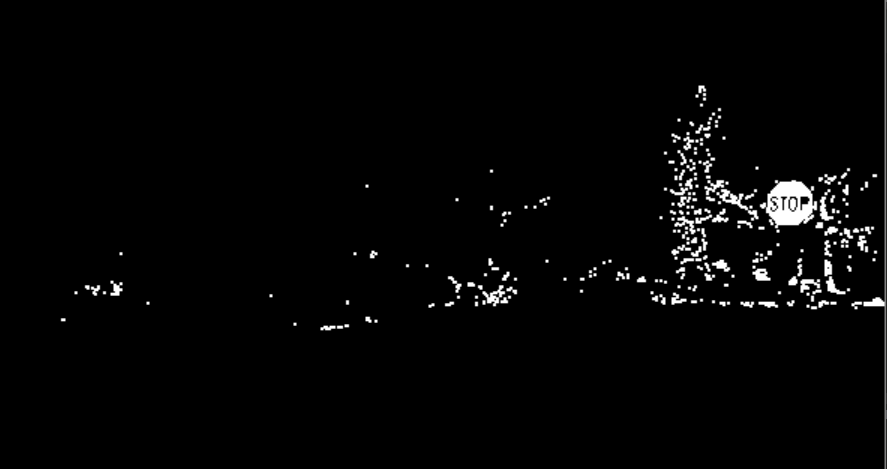
\includegraphics[width=70mm]{segment_trees.png}}

\centerline{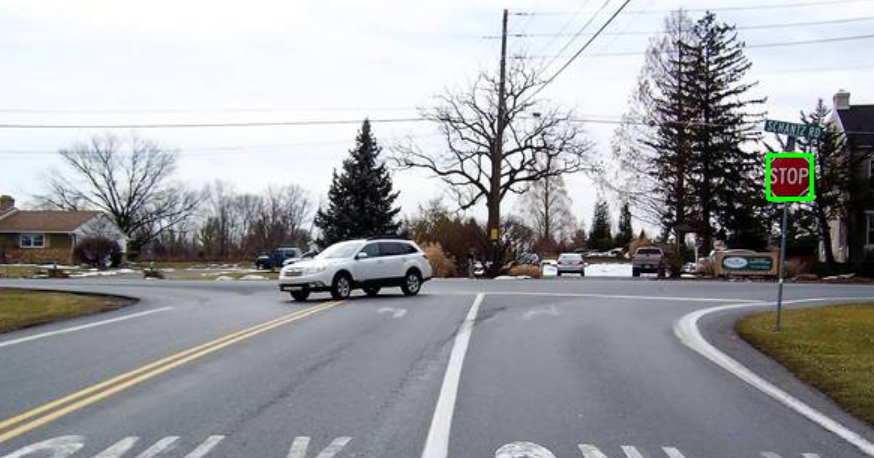
\includegraphics[width=70mm]{box_trees.png}}
\caption{Color segmentation mask and successful stop sign detection of an image with one stop sign}
\end{figure}

\begin{figure}[H]

\centerline{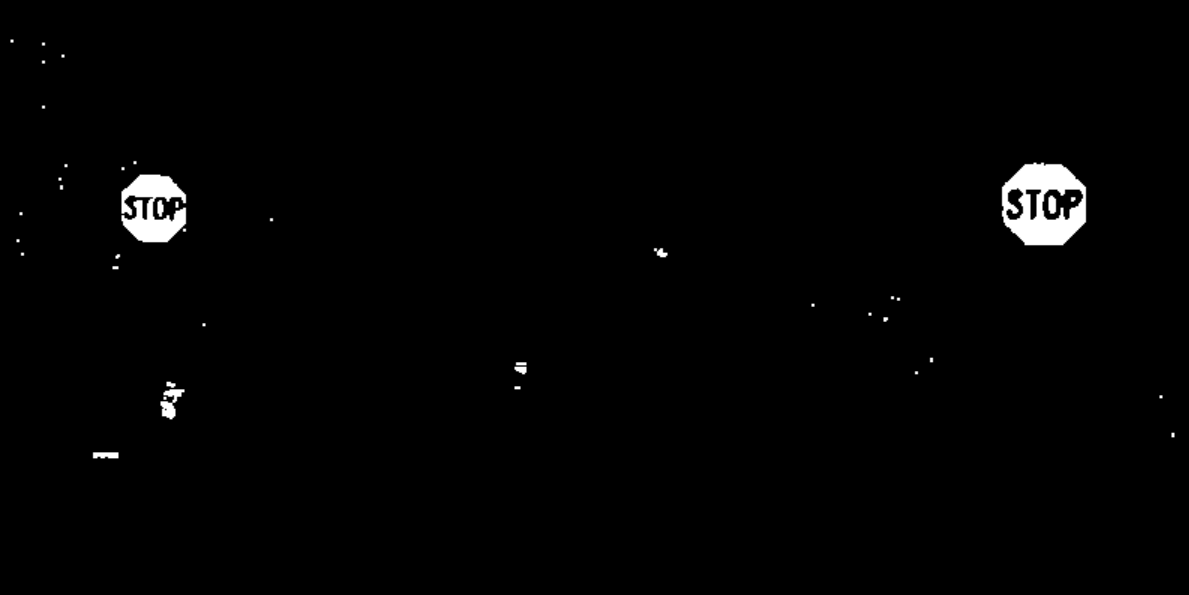
\includegraphics[width=70mm]{double_stop_sign.png}}

\centerline{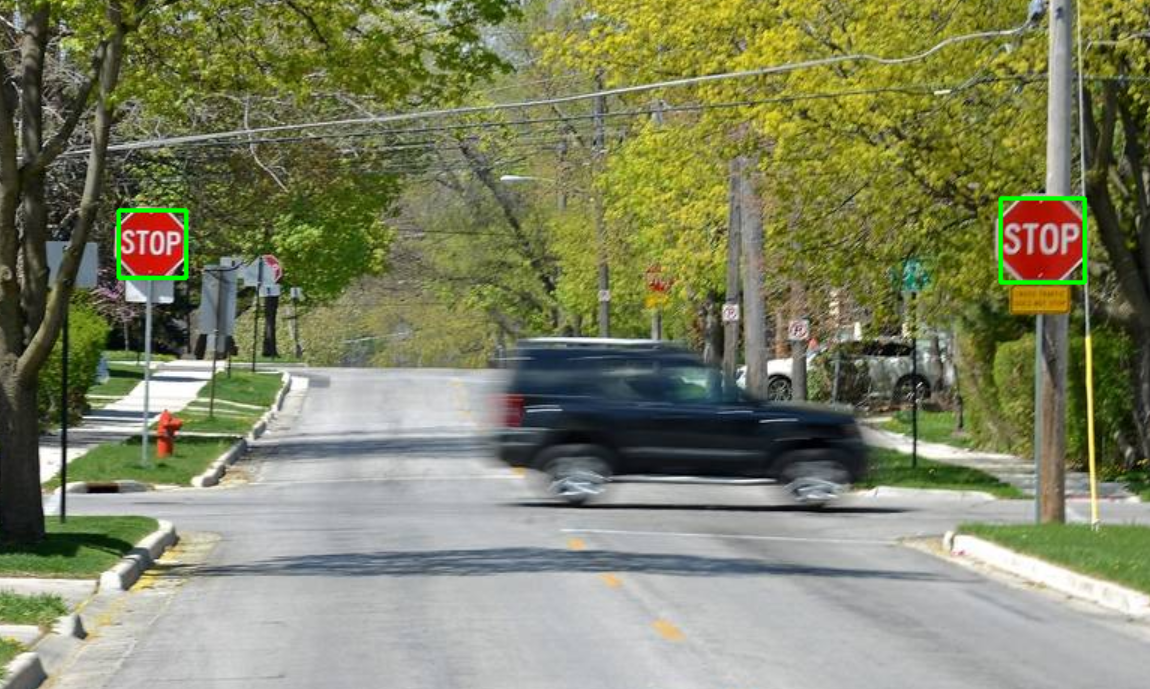
\includegraphics[width=70mm]{double_stop_sign_boxes.png}}
\caption{Color segmentation mask and successful stop sign detection of an image with two stop signs}
\end{figure}

\begin{figure}[H]
\centerline{
\includegraphics[width=70mm]{obstruct_mask.png}}

\centerline{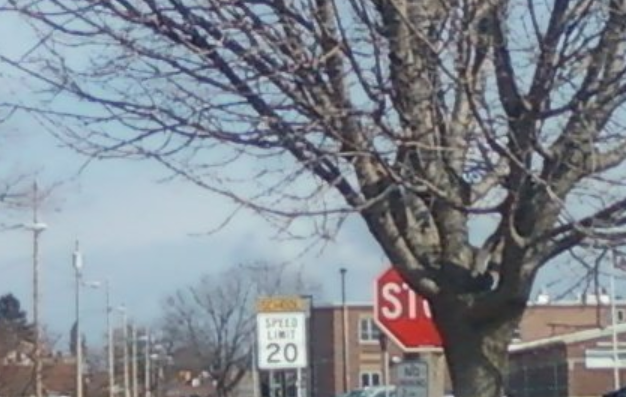
\includegraphics[width=70mm]{obstruct_boxes.png}}
\caption{Color segmentation mask and unsuccessful stop sign detection due to occlusion}
\end{figure}

I would be interested to replicate this paper but with the use of a Gaussian mixture model for color segmentation to compare the results. The color segmentation of the model detailed in this paper was quite good, but struggled in some more difficult images. I anticipate a Gaussian mixture model may be more successful in these harder cases.


\begin{thebibliography}{00}
\bibitem{b1} Dubai's Autonomous Transportation Strategy. (2016, April 25). Retrieved from https://www.dubaifuture.gov.ae/our-initiatives/dubais-autonomous-transportation-strategy.
\bibitem{b2} Allianz Global Assistance survey finds fewer Americans interested in autonomous vehicles. (2018, September 19). Retrieved February 1, 2020, from https://www.greencarcongress.com/2018/09/20180919-allianz.html
\bibitem{b3} jdoepfert/roipoly.py. (2019, September 29). Retrieved February 1, 2020, from https://github.com/jdoepfert/roipoly.py

\end{thebibliography}
\vspace{12pt}


\end{document}
